\documentclass[aspectratio=169,xcolor=table]{beamer}
\usepackage{hyperref}
\usepackage{tikz}
\usepackage{graphicx}
\usepackage{graphbox}
\usepackage{siunitx}
\usepackage[maxcitenames=6, url=false,doi=false]{biblatex}
\usepackage{subcaption}
\usepackage[outputdir=_build,draft=false]{minted}
\usepackage{pdfpc}

\usepackage{lmodern}
\usepackage{libertine}
\renewcommand\ttdefault{lmtt}

\usepackage{dirtree}
% Unsaturated
% \definecolor{cnt}{HTML}{C7C1C2}
% \definecolor{dir}{HTML}{DBDCE8}
% \definecolor{rev}{HTML}{E7F2F2}
% \definecolor{rel}{HTML}{FFFCCD}
% \definecolor{snp}{HTML}{F5F5F5}
% \definecolor{ori}{HTML}{FFFFFF}

% Saturated, darkened
% \definecolor{cnt}{HTML}{BBA3A7}
% \definecolor{dir}{HTML}{B7BAD9}
% \definecolor{rev}{HTML}{C3E3E3}
% \definecolor{rel}{HTML}{FFF89A}
% \definecolor{snp}{HTML}{E3E3E3}
% \definecolor{ori}{HTML}{FFFFFF}

% Saturated, darkened, improved
\definecolor{cnt}{HTML}{BFA6AA}
\definecolor{dir}{HTML}{CFD2F2}
\definecolor{rev}{HTML}{C3E3E3}
\definecolor{rel}{HTML}{FFF9A3}
\definecolor{snp}{HTML}{E3E3E3}
\definecolor{ori}{HTML}{FFFFFF}

\makeatletter
\pgfkeys{/tikz/.cd,
  tab height/.initial=3pt,
  tab width/.initial=10pt,
  tab slope/.initial=1.5pt,
  cover xoff/.initial=5pt,
  cover yoff/.initial=2pt,
}
%% Note: use '\setlength{\pgf@xd}{\pgf@xb}' rather than '\pgf@xd=\pgf@xb'
%% ??? for some reason \pgf@ytt etc. didn't work, but \pgf@ytt does
\newlength\pgf@ytt
\newlength\pgf@xe
\newlength\pgf@xf
\newlength\pgf@xg
\newlength\pgf@yg
\newlength\pgf@xh
%% this didn't work
\newlength\pgf@xo  %% note: \pgf@xx is pre-defined by pgf to mean something

%% from 95.2 Communicating with the Basic Layer via Macros
% \newdimen\pgf@xta \newdimen\pgf@xtb \newdimen\pgf@ytt
% \newdimen\pgf@xoa \newdimen\pgf@xob \newdimen\pgf@yoo
\pgfdeclareshape{document}{ % or 'directory'
  %% this is nearly a rectangle
  \inheritsavedanchors[from=rectangle]
  \inheritanchorborder[from=rectangle]
  \inheritanchor[from=rectangle]{center}
  \inheritanchor[from=rectangle]{north}
  \inheritanchor[from=rectangle]{south}

  \savedmacro\tabheight{%
    \edef\tabheight{\pgfkeysvalueof{/tikz/tab height}}%
  }
  \savedmacro\tabwidth{%
    \edef\tabwidth{\pgfkeysvalueof{/tikz/tab width}}%
  }
  \savedmacro\tabslope{%
    \edef\tabslope{\pgfkeysvalueof{/tikz/tab slope}}%
  }
  \savedmacro\coverxoff{%
    \edef\coverxoff{\pgfkeysvalueof{/tikz/cover xoff}}%
  }
  \savedmacro\coveryoff{%
    \edef\coveryoff{\pgfkeysvalueof{/tikz/cover yoff}}%
  }
  %% this didn't work; probably needs \pgf@process somewhere...
  % \setlength{\pgf@xo}{\coverxoff}
  % \setlength{\pgf@xo}{0.5\pgf@xo}

  %% this didn't work either
  % \setlength{\pgf@xo}{2pt}
  % \advance\pgf@xo by \coverxoff\relax

  %% this didn't work either
  % \pgf@xx=0pt
  % \advance\pgf@xx by \coverxoff\relax
  % \pgf@xx=0.5\pgf@xx

  %% fallback, so this at least compile
  %% but moves text, because \pgf@xx is sed for node contents positioning
  % \pgf@xx=2pt % this should be 0.5 of \coverxoff

  % \inheritanchor[from=rectangle]{west}
  \anchor{west}{
    \pgf@process{\northeast}%
    \pgf@ya=.5\pgf@y%
    \pgf@process{\southwest}%
    \pgf@y=.5\pgf@y%
    % \advance\pgf@y by  \pgf@ya%
    % \advance\pgf@x by -2pt%
  }
  % \inheritanchor[from=rectangle]{east}
  \anchor{east}{%
    \pgf@process{\southwest}%
    \pgf@ya=.5\pgf@y%
    \pgf@process{\northeast}%
    \pgf@y=.5\pgf@y%
    % \advance\pgf@y by  \pgf@ya%
    % \advance\pgf@x by  2pt%
  }
  \backgroundpath{% this is new
    %% store lower left in xa/ya and upper right in xb/yb
    \southwest \pgf@xa=\pgf@x \pgf@ya=\pgf@y
    \northeast \pgf@xb=\pgf@x \pgf@yb=\pgf@y
    %% correction due to open front cover
    % \advance\pgf@xa by -2pt
    % \advance\pgf@xb by -2pt
    %%
    %% compute edges of the "divider tab" in the back cover
    %%
    \setlength{\pgf@ytt}{\pgf@yb}
    \advance\pgf@ytt by \tabheight
    \setlength{\pgf@xe}{\pgf@xa}
    \advance\pgf@xe by \tabwidth % or make it dependent on box width
    \setlength{\pgf@xf}{\pgf@xe}
    \advance\pgf@xf by \tabslope % or make it dependent on divider height
    %%
    %% compute edges of second cover of a folder ("open" cover)
    %%
    \setlength{\pgf@xg}{\pgf@xa}
    \advance\pgf@xg by \coverxoff % perhaps as an angle of open
    \setlength{\pgf@xh}{\pgf@xb}
    \advance\pgf@xh by \coverxoff
    \setlength{\pgf@yg}{\pgf@yb}
    \advance\pgf@yg by-\coveryoff % perhaps as an angle of open
    %%
    %% construct main path
    \pgfpathmoveto{\pgfpoint{\pgf@xa}{\pgf@ya}}
    \pgfpathlineto{\pgfpoint{\pgf@xa}{\pgf@ytt}}
    \pgfpathlineto{\pgfpoint{\pgf@xe}{\pgf@ytt}}
    \pgfpathlineto{\pgfpoint{\pgf@xf}{\pgf@yb}}
    \pgfpathlineto{\pgfpoint{\pgf@xb}{\pgf@yb}}
    \pgfpathlineto{\pgfpoint{\pgf@xb}{\pgf@ya}} % break for open cover
    \pgfpathmoveto{\pgfpoint{\pgf@xb}{\pgf@ya}}
    % \pfgpathlineto{\pgfpoint{\pgf@xa}{\pgf@ya}} % ??? causes error ???
    \pgfpathclose
    %% construct secondary path
    \pgfpathmoveto{\pgfpoint{\pgf@xa}{\pgf@ya}}
    % \pgfpathlineto{\pgfpoint{\pgf@xg}{\pgf@yg}}
    % \pgfpathlineto{\pgfpoint{\pgf@xh}{\pgf@yg}}
    \pgfpathlineto{\pgfpoint{\pgf@xb}{\pgf@ya}}
    \pgfpathclose
  }
}
\makeatother

\usetikzlibrary{calc}
\usepackage{etoolbox}

\pgfdeclarelayer{background}
\pgfdeclarelayer{foreground}
\pgfdeclarelayer{sankeydebug}
\pgfsetlayers{background,main,foreground,sankeydebug}

\newif\ifsankeydebug

\newenvironment{sankeydiagram}[1][]{

  \def\sankeyflow##1##2{% sn, en
    \path[sankey fill]
    let
    \p1=(##1.north east),\p2=(##1.south east),
    \n1={atan2(\y1-\y2, \x1-\x2)-90},
    \p3=(##2.north west),\p4=(##2.south west),
    \n2={atan2(\y3-\y4, \x3-\x4)+90}
    in
    (\p1) to[out=\n1,in=\n2] (\p3) --
    (\p4) to[in=\n1,out=\n2] (\p2) -- cycle;
    \draw[sankey draw]
    let
    \p1=(##1.north east),\p2=(##1.south east),
    \n1={atan2(\y1-\y2, \x1-\x2)-90},
    \p3=(##2.north west),\p4=(##2.south west),
    \n2={atan2(\y3-\y4, \x3-\x4)+90}
    in
    (\p1) to[out=\n1,in=\n2] (\p3)
    (\p4) to[in=\n1,out=\n2] (\p2);
  }


  \tikzset{
    sankey tot length/.store in=\sankeytotallen,
    sankey tot quantity/.store in=\sankeytotalqty,
    sankey min radius/.store in=\sankeyminradius,
    sankey arrow length/.store in=\sankeyarrowlen,
    sankey debug/.is if=sankeydebug,
    sankey debug=false,
    sankey flow/.style={
      to path={
        \pgfextra{
          \pgfinterruptpath
          \edef\sankeystart{\tikztostart}
          \edef\sankeytarget{\tikztotarget}
          \sankeyflow{\sankeystart}{\sankeytarget}
          \endpgfinterruptpath
        }
      },
    },
    sankey node/.style={
      inner sep=0,minimum height={sankeyqtytolen(##1)},
      minimum width=0,draw=none,line width=0pt,
    },
    % sankey angle
    sankey angle/.store in=\sankeyangle,
    % sankey default styles
    sankey fill/.style={line width=0pt,fill,white},
    sankey draw/.style={draw=black,line width=.4pt},
  }

  \newcommand\sankeynode[4]{%prop,orientation,name,pos
    \node[sankey node=##1,rotate=##2] (##3) at (##4) {};
    \ifsankeydebug
    \begin{pgfonlayer}{sankeydebug}
      \draw[red,|-|] (##3.north west) -- (##3.south west);
      \pgfmathsetmacro{\len}{sankeyqtytolen(##1)/3}
      \draw[red] (##3.west)
      -- ($(##3.west)!\len pt!90:(##3.south west)$)
      node[font=\tiny,text=black] {##3};
    \end{pgfonlayer}
    \fi
  }

  \newcommand\sankeynodestart[4]{%prop,orientation,name,pos
    \sankeynode{##1}{##2}{##3}{##4}
    \begin{scope}[shift={(##3)},rotate=##2]
      \path[sankey fill]
      (##3.north west) -- ++(-\sankeyarrowlen,0)
      -- ([xshift=-\sankeyarrowlen/6]##3.west)
      -- ([xshift=-\sankeyarrowlen]##3.south west)
      -- (##3.south west) -- cycle;
      \path[sankey draw]
      (##3.north west) -- ++(-\sankeyarrowlen,0)
      -- ([xshift=-\sankeyarrowlen/6]##3.west)
      -- ([xshift=-\sankeyarrowlen]##3.south west)
      -- (##3.south west);
    \end{scope}
  }

  \newcommand\sankeynodeend[4]{%prop,orientation,name,pos
    \sankeynode{##1}{##2}{##3}{##4}
    \begin{scope}[shift={(##3)},rotate=##2]
      \path[sankey fill]
      (##3.north east)
      -- ([xshift=\sankeyarrowlen]##3.east)
      -- (##3.south west) -- cycle;
      \path[sankey draw]
      (##3.north east)
      -- ([xshift=\sankeyarrowlen]##3.east)
      -- (##3.south west);
    \end{scope}
  }

  \newcommand\sankeyadvance[3][]{%newname,name,distance
    \edef\name{##2}
    \ifstrempty{##1}{
      \def\newname{##2}
      \edef\name{##2-old}
      \path [late options={name=##2,alias=\name}];
    }{
      \def\newname{##1}
    }
    \path
    let
    % sankey node angle
    \p1=(##2.north east),
    \p2=(##2.south east),
    \n1={atan2(\y1-\y2, \x1-\x2)-90},
    % sankey prop
    \p3=($(\p1)-(\p2)$),
    \n2={sankeylentoqty(veclen(\x3,\y3))},
    % next position
    \p4=($(##2.east)!##3!-90:(##2.north east)$)
    in
    \pgfextra{
      \pgfmathsetmacro{\prop}{\n2}
      \pgfinterruptpath
      \sankeynode{\prop}{\n1}{\newname}{\p4}
      \path (\name) to[sankey flow] (\newname);
      \endpgfinterruptpath
    };
  }

  \newcommand\sankeyturn[3][]{%newname,name,angle
    \edef\name{##2}
    \ifstrempty{##1}{
      \def\newname{##2}
      \edef\name{##2-old}
      \path [late options={name=##2,alias=\name}];
    }{
      \def\newname{##1}
    }
    \ifnumgreater{##3}{0}{
      \path
      let
      % sankey node angle
      \p1=(##2.north east),
      \p2=(##2.south east),
      \p3=($(\p1)!-\sankeyminradius!(\p2)$),
      \n1={atan2(\y1-\y2, \x1-\x2)-90},
      % sankey prop
      \p4=($(\p1)-(\p2)$),
      \n2={sankeylentoqty(veclen(\x4,\y4))},
      \p5=(##2.east),
      \p6=($(\p3)!1!##3:(\p5)$)
      in
      \pgfextra{
        \pgfmathsetmacro{\prop}{\n2}
        \pgfinterruptpath
        % \fill[red] (\p3) circle (2pt);
        % \fill[blue](\p6) circle (2pt);
        \sankeynode{\prop}{\n1+##3}{\newname}{\p6}
        \path (\name) to[sankey flow] (\newname);
        \endpgfinterruptpath
      };
    }{
      \path
      let
      % sankey node angle
      \p1=(##2.south east),
      \p2=(##2.north east),
      \p3=($(\p1)!-\sankeyminradius!(\p2)$),
      \n1={atan2(\y1-\y2, \x1-\x2)+90},
      % sankey prop
      \p4=($(\p1)-(\p2)$),
      \n2={sankeylentoqty(veclen(\x4,\y4))},
      \p5=(##2.east),
      \p6=($(\p3)!1!##3:(\p5)$)
      in
      \pgfextra{
        \pgfmathsetmacro{\prop}{\n2}
        \pgfinterruptpath
        % \fill[red] (\p3) circle (2pt);
        % \fill[blue](\p6) circle (2pt);
        \sankeynode{\prop}{\n1+##3}{\newname}{\p6}
        \path (\name) to[sankey flow] (\newname);
        \endpgfinterruptpath
      };
    }
  }

  \newcommand\sankeyfork[2]{%name,list of forks
    \def\name{##1}
    \def\listofforks{##2}
    \xdef\sankeytot{0}
    \path 
    let
    % sankey node angle
    \p1=(\name.north east),
    \p2=(\name.south east),
    \n1={atan2(\y1-\y2, \x1-\x2)-90},
    % sankey prop
    \p4=($(\p1)-(\p2)$),
    \n2={sankeylentoqty(veclen(\x4,\y4))}
    in
    \pgfextra{
      \pgfmathsetmacro{\iprop}{\n2}
    }
    \foreach \prop/\name[count=\c] in \listofforks {
      let
      \p{start \name}=($(\p1)!\sankeytot/\iprop!(\p2)$),
      \n{nexttot}={\sankeytot+\prop},
      \p{end \name}=($(\p1)!\n{nexttot}/\iprop!(\p2)$),
      \p{mid \name}=($(\p{start \name})!.5!(\p{end \name})$)
      in
      \pgfextra{
        \xdef\sankeytot{\n{nexttot}}
        \pgfinterruptpath
        \sankeynode{\prop}{\n1}{\name}{\p{mid \name}}
        \endpgfinterruptpath
      }
    }
    \pgfextra{
      \pgfmathsetmacro{\diff}{abs(\iprop-\sankeytot)}
      \pgfmathtruncatemacro{\finish}{\diff<0.01?1:0}
      \ifnumequal{\finish}{1}{}{
        \message{*** Warning: bad sankey fork (maybe)...}
        \message{\iprop-\sankeytot}
      }
    };
  }

  \tikzset{
    % default values,
    declare function={
      sankeyqtytolen(\qty)=\qty/\sankeytotalqty*\sankeytotallen;
      sankeylentoqty(\len)=\len/\sankeytotallen*\sankeytotalqty;
    },
    sankey tot length=100pt,
    sankey tot quantity=100,
    sankey min radius=30pt,%
    sankey arrow length=10pt,%
    % user values
    #1}
}{
}

\input{../tikz/swh.tikzstyles}
\input{../tikz/swh.tikzdefs}

\definecolor{palegrey}{RGB}{242, 242, 244}
\definecolor{SwhLightRed}{cmyk}{.0,.89,.84,.07}

\setbeamercolor{background canvas}{bg=palegrey}
\useinnertheme{rounded}
\useoutertheme{shadow}
% \useoutertheme{infolines}
\usecolortheme{orchid}
\usecolortheme{whale}
\usecolortheme[named=SwhLightRed]{structure}

\setbeamerfont{footline}{series=\bfseries}
\setbeamertemplate{page number in head/foot}[totalframenumber]
\setbeamertemplate{navigation symbols}{}
\setbeamertemplate{bibliography item}[article]

\rowcolors[]{1}{blue!10}{blue!05}

\titlegraphic{%
    \hfill%
    
\includegraphics[align=c, width=0.3\textwidth]{../img/frontmatter/uni_paris}%
    \hfill%
    
\includegraphics[align=c, width=0.20\textwidth]{../img/frontmatter/inria.pdf}%
    \hfill%
    
\includegraphics[align=c, width=0.3\textwidth]{../img/frontmatter/SWH-logo}
    \hfill%
}

\AtBeginSection[]{%
    \begin{frame}
        \frametitle{Table of Contents}
        \tableofcontents[currentsection]
    \end{frame}
}

\setbeamertemplate{headline}{}


\title[Organizing the graph of public software development]{Organizing the graph of public software development for large-scale mining}
\subtitle{PhD Thesis Defense}
\author{Antoine \textsc{Pietri}}
\institute{Inria, Paris}
\date{November 5, 2021}

\hypersetup{%
    pdfauthor={Antoine Pietri},
    pdftitle={Organizing the graph of public software development for
        large-scale mining},
    pdfkeywords={empirical software engineering, source code, open source
        software, version control system, digital preservation, graph topology,
        graph
    compression},
    pdflang={English}
}


\begin{document}
    \maketitle

    \begin{frame}{Outline}
        \tableofcontents
    \end{frame}

    \section{Introduction: Universal Mining in Software Heritage}
    % presentation
    % universal software mining

    \section{Data Model}

    \begin{frame}
        \frametitle{A source code directory}

        \begin{columns}
            \column{.30\textwidth}
            \begin{figure}
                \begin{minipage}{\textwidth}
                \dirtree{%
                    .1 /.
                        .2 src.
                            .3 evalexpr.c.
                            .3 parser.
                                .4 ast.c.
                                .4 parser.c.
                                .4 lexer.c.
                        .2 tests.
                            .3 eval.c.
                            .3 operands.c.
                }
            \end{minipage}
            \end{figure}
            \column{.70\textwidth}
            \begin{figure}
                \centering
                \scalebox{0.9}{\begin{tikzpicture}[scale=2, font=\footnotesize]
	\begin{pgfonlayer}{nodelayer}
		\node [style=directory] (9) at (3, -2) {};
		\node [style=directory] (10) at (1, -2) {};
		\node [style=directory] (14) at (1.5, -3) {};
		\node [style=content] (16) at (1.5, -4) {};
		\node [style=content] (17) at (2.25, -4) {};
		\node [style=content] (18) at (0.75, -4) {};
		\node [style=content] (19) at (0, -3) {};
		\node [style=directory] (20) at (2, -1.5) {};
		\node [style=content] (21) at (2.5, -3) {};
		\node [style=content] (22) at (3.5, -3) {};
	\end{pgfonlayer}
	\begin{pgfonlayer}{edgelayer}
		\draw [style=arrow] (20) to node [above,sloped] {src} (10);
		\draw [style=arrow] (10) to node [above,sloped] {evalexpr.c} (19);
		\draw [style=arrow] (10) to node [above,sloped] {parser} (14);
		\draw [style=arrow] (14) to node [above,sloped] {ast.c} (16);
		\draw [style=arrow] (14) to node [above,sloped] {lexer.c} (17);
		\draw [style=arrow] (14) to node [above,sloped] {parser.c} (18);
		\draw [style=arrow] (20) to node [above,sloped] {tests} (9);
		\draw [style=arrow] (9) to node [above,sloped] {parser.c} (21);
		\draw [style=arrow] (9) to node [above,sloped] {operands.c} (22);
	\end{pgfonlayer}
\end{tikzpicture}
}
            \end{figure}
        \end{columns}
    \end{frame}

    \begin{frame}
        \frametitle{Revisions}
        % Parallel history
        \begin{block}{}
            \begin{itemize}
                \item \textbf{Revisions} (or ``commits'') keep track of
                    successive states of a source directory.
            \end{itemize}
        \end{block}
        \vfill
        \begin{figure}
            \centering
            \scalebox{0.8}{\begin{tikzpicture}[scale=1.5, font={\small}]
	\begin{pgfonlayer}{nodelayer}
		\node [style=directory] (10) at (2, -1.5) {};
		\node [style=directory] (14) at (2, -2.25) {};
		\node [style=content] (16) at (2, -3) {};
		\node [style=content] (17) at (2.5, -3) {};
		\node [style=content] (18) at (1.5, -3) {};
		\node [style=content] (19) at (1.25, -2.25) {};
		\node [style=directory] (20) at (2, -0.75) {};
		\node [style=revision, label={[align=center]\textbf{Second revision} \\ Add parser}] (23) at (2, 0) {};
		\node [style=revision, label={[align=center]\textbf{Third revision} \\ Add tests}] (24) at (5, 0) {};
		\node [style=directory] (25) at (5.5, -1.5) {};
		\node [style=directory] (26) at (4.5, -1.5) {};
		\node [style=directory] (27) at (4.5, -2.25) {};
		\node [style=content] (28) at (4.5, -3) {};
		\node [style=content] (29) at (5, -3) {};
		\node [style=content] (30) at (4, -3) {};
		\node [style=content] (31) at (3.75, -2.25) {};
		\node [style=directory] (32) at (5, -0.75) {};
		\node [style=content] (33) at (5.25, -2.25) {};
		\node [style=content] (34) at (5.75, -2.25) {};
		\node [style=revision, label={[align=center]\textbf{First revision} \\ Initial prototype}] (35) at (-1, 0) {};
		\node [style=directory] (36) at (-1, -0.75) {};
		\node [style=content] (37) at (-1, -1.5) {};
	\end{pgfonlayer}
	\begin{pgfonlayer}{edgelayer}
		\draw [style=arrow] (10) to (14);
		\draw [style=arrow] (14) to (16);
		\draw [style=arrow] (14) to (17);
		\draw [style=arrow] (20) to node [above, sloped] {\tiny src} (10);
		\draw [style=arrow] (10) to (19);
		\draw [style=arrow] (14) to (18);
		\draw [style=arrow] (23) to (20);
		\draw [style=arrow] (24) to (23);
		\draw [style=arrow] (26) to (27);
		\draw [style=arrow] (27) to (28);
		\draw [style=arrow] (27) to (29);
		\draw [style=arrow] (32) to node [above, sloped] {\tiny src} (26);
		\draw [style=arrow] (32) to node [above, sloped] {\tiny tests} (25);
		\draw [style=arrow] (26) to (31);
		\draw [style=arrow] (27) to (30);
		\draw [style=arrow] (25) to (33);
		\draw [style=arrow] (25) to (34);
		\draw [style=arrow] (24) to (32);
		\draw [style=arrow] (23) to (35);
		\draw [style=arrow] (35) to (36);
		\draw [style=arrow] (36) to (37);
	\end{pgfonlayer}
\end{tikzpicture}
}
        \end{figure}
    \end{frame}

    \begin{frame}
        \frametitle{Branching and merging}

        \begin{block}{}
            \begin{itemize}
                \item ``Branching'' allows multiple developers to work on
                    different features simultaneously.
                \item ``Merging'' is used to integrate their respective changes
                    back to a shared state.
            \end{itemize}
        \end{block}
        \vfill
        \begin{figure}
            \centering
            \scalebox{0.8}{\begin{tikzpicture}
	\begin{pgfonlayer}{nodelayer}
		\node [style=revision] (0) at (0, 0) {};
		\node [style=revision, label={[align=center]below:Branching\\revision}] (1) at (2, 0) {};
		\node [style=revision] (2) at (4, 0) {};
		\node [style=revision] (3) at (3, 1) {};
		\node [style=revision] (4) at (4.75, 1) {};
		\node [style=revision] (5) at (6, 0) {};
		\node [style=revision, label={[align=center]below:Merge\\revision}] (6) at (8, 0) {};
		\node [style=revision] (7) at (6.5, 1) {};
		\node [style=revision] (8) at (9.5, 0) {};
	\end{pgfonlayer}
	\begin{pgfonlayer}{edgelayer}
		\draw [style=arrow] (1) to (0);
		\draw [style=arrow] (3) to (1);
		\draw [style=arrow] (4) to (3);
		\draw [style=arrow] (7) to (4);
		\draw [style=arrow] (6) to (7);
		\draw [style=arrow] (2) to (1);
		\draw [style=arrow] (5) to (2);
		\draw [style=arrow] (6) to (5);
		\draw [style=arrow] (8) to (6);
	\end{pgfonlayer}
\end{tikzpicture}
}
        \end{figure}
    \end{frame}

    \begin{frame}
        \frametitle{Branches}
        \begin{block}{}
            \begin{itemize}
                \item \textbf{Branches} are dynamic pointers to revisions,
                    using mnemonic names to keep track of their purpose.
                \item Branch pointers move when more revisions are added to the
                    branch.
            \end{itemize}
        \end{block}
        % TODO: animate
        \vfill
        \begin{figure}
            \centering
            \scalebox{0.8}{\begin{tikzpicture}
	\begin{pgfonlayer}{nodelayer}
		\node [style=revision] (0) at (0, 0) {};
		\node [style=revision] (1) at (2, 0) {};
		\node [style=revision] (2) at (4, 0) {};
		\node [style=revision] (3) at (6, 0) {};
		\node [style=revision] (4) at (8, 0) {};
		\node [style=revision] (5) at (3, 1) {};
		\node [style=revision] (6) at (5, 1) {};
		\node [style=revision] (7) at (5, -1) {};
		\node [style=revision] (8) at (7, -1) {};
		\node [style=branch] (9) at (5, 2.25) {feature-parser};
		\node [style=branch] (10) at (8, 2.25) {main};
		\node [style=branch] (11) at (9, 1) {test-ci};
		\node [style=revision] (12) at (9, -1) {};
	\end{pgfonlayer}
	\begin{pgfonlayer}{edgelayer}
		\draw [style=arrow] (1) to (0);
		\draw [style=arrow] (2) to (1);
		\draw [style=arrow] (3) to (2);
		\draw [style=arrow] (4) to (3);
		\draw [style=arrow] (5) to (1);
		\draw [style=arrow] (6) to (5);
		\draw [style=arrow] (7) to (2);
		\draw [style=arrow] (8) to (7);
		\draw [style=dashed arrow] (9) to (6);
		\draw [style=dashed arrow] (10) to (4);
		\draw [style=dashed arrow] (11) to (12);
		\draw [style=arrow] (12) to (8);
	\end{pgfonlayer}
\end{tikzpicture}
}
        \end{figure}
    \end{frame}

    \begin{frame}
        \frametitle{Releases}
        \begin{block}{}
            \begin{itemize}
                \item \textbf{Releases} (or ``tags'') point to specific
                    milestones in the development history.
                \item They have mnemonic names, usually representing the
                    software version.
            \end{itemize}
        \end{block}
        % TODO: animate
        \vfill
        \begin{figure}
            \centering
            \scalebox{0.8}{\begin{tikzpicture}
	\begin{pgfonlayer}{nodelayer}
		\node [style=revision] (0) at (0, 0) {};
		\node [style=revision] (1) at (2, 0) {};
		\node [style=revision] (2) at (4, 0) {};
		\node [style=revision] (3) at (6, 0) {};
		\node [style=revision] (4) at (8, 0) {};
		\node [style=revision] (7) at (3, -1) {};
		\node [style=revision] (8) at (5, -1) {};
		\node [style=branch] (10) at (10, 2) {main};
		\node [style=revision] (12) at (7, -1) {};
		\node [style=revision] (13) at (10, 0) {};
		\node [style=revision] (14) at (6, -2) {};
		\node [style=revision] (15) at (8, -2) {};
		\node [style=release, label={\textbf{v2.0}}] (16) at (8, 2) {};
		\node [style=release, label={\textbf{v1.0}}] (17) at (4, 2) {};
	\end{pgfonlayer}
	\begin{pgfonlayer}{edgelayer}
		\draw [style=arrow] (1) to (0);
		\draw [style=arrow] (2) to (1);
		\draw [style=arrow] (3) to (2);
		\draw [style=arrow] (4) to (3);
		\draw [style=arrow] (8) to (7);
		\draw [style=arrow] (12) to (8);
		\draw [style=arrow] (4) to (12);
		\draw [style=arrow] (7) to (1);
		\draw [style=dashed arrow] (10) to (13);
		\draw [style=arrow] (13) to (4);
		\draw [style=arrow] (14) to (8);
		\draw [style=arrow] (15) to (14);
		\draw [style=dashed arrow] (16) to (4);
		\draw [style=dashed arrow] (17) to (2);
	\end{pgfonlayer}
\end{tikzpicture}
}
        \end{figure}
    \end{frame}

    \begin{frame}
        \frametitle{Deduplication}
        \begin{block}{}
            \begin{itemize}
                \item Lots of frozen states $\Rightarrow$ lots of copies of
                    objects
                \item Most objects stay identical from one revision to another
                \pause
                \item We can identify \& deduplicate them with
                    \textbf{cryptographic hash functions}.
            \end{itemize}
        \end{block}
        \vfill
        \begin{figure}
            \centering
            \scalebox{0.8}{\begin{tikzpicture}
    \node [
        shape=rectangle, draw=black, align=left, font=\tiny,
        label={[above]Input text}
    ] (input) at (0, 0)
        {%
            L'argoumante était églomatique et s'impliquait \\
            beaucoup plus qu'à l'exparité. Le plus déjà se \\
            plussissait. Plus qu'à l'exparité s'étrangent et se \\
            consument les pregmes endiablés de la légume.
    };

    \node [
        shape=ellipse, draw=black, align=left, fill=cyan!25,
        label={[above,align=center]Cryptographic \\ hash function}
    ] (hash) at (5.5, 0) {SHA-256};

    \node [
        shape=rectangle, draw=black, align=center, font=\footnotesize,
        label={[above]Result hash}
    ] (output) at (10, 0) {%
        % \texttt{7a50e30ada8f09b2}%
        % \texttt{24d348d314de4c09} \\
        % \texttt{ae0ebcb443334442}%
        % \texttt{70cc832ebfc6bc0c}

        \texttt{7a50e30ada8f09b224d34} \\
        \texttt{8d314de4c09ae0ebcb443} \\
        \texttt{33444270cc832ebfc6bc0c}
    };

    \draw[->, >=Stealth] (input) to (hash);
    \draw[->, >=Stealth] (hash) to (output);
\end{tikzpicture}
}
        \end{figure}
        \begin{block}{Cryptographic hash functions (SHA-1, SHA-256, BLAKE2, …)}
            \begin{itemize}
                \item Associates an arbitrary input with a
                    \emph{unique\footnote{Terms and conditions apply.}
                    identifier} called a \textbf{hash}
                \item Check if two objects are identical in O(1).
            \end{itemize}
        \end{block}
    \end{frame}

    \begin{frame}
        \frametitle{Deduplicating files}
        \begin{block}{}
            \begin{itemize}
                \item VCSs identify each file via their unique hash
                \item Identical files are \emph{deduplicated} (= shared) from
                    one revision to another.
            \end{itemize}
        \end{block}
        % TODO: animate
        \vfill
        \begin{figure}
            \centering
            \scalebox{0.8}{\begin{tikzpicture}[scale=1.5, font={\small}]
	\begin{pgfonlayer}{nodelayer}
		\node [style=directory] (10) at (2, -1.5) {};
		\node [style=directory] (14) at (2, -2.25) {};
		\node [style=content] (16) at (2, -3.5) {C};
		\node [style=content] (17) at (2.5, -3.5) {D};
		\node [style=content] (18) at (1.5, -3.5) {B};
		\node [style=content, fill=white, dotted] (19) at (1.25, -2.25) {A};
		\node [style=directory] (20) at (2, -0.75) {};
		\node [style=revision] (23) at (2, 0) {};
		\node [style=revision] (24) at (5, 0) {};
		\node [style=directory] (25) at (5.5, -1.5) {};
		\node [style=directory] (26) at (4.5, -1.5) {};
		\node [style=directory] (27) at (4.5, -2.25) {};
		\node [style=content, fill=white, dotted] (28) at (4.5, -3.5) {C};
		\node [style=content, fill=white, dotted] (29) at (5, -3.5) {D};
		\node [style=content, fill=white, dotted] (30) at (4, -3.5) {B};
		\node [style=content, fill=white, dotted] (31) at (3.75, -2.25) {A};
		\node [style=directory] (32) at (5, -0.75) {};
		\node [style=content] (33) at (5.25, -2.25) {E};
		\node [style=content] (34) at (5.75, -2.25) {F};
		\node [style=revision] (35) at (-1, 0) {};
		\node [style=directory] (36) at (-1, -0.75) {};
		\node [style=content] (37) at (-1, -1.5) {A};
	\end{pgfonlayer}
	\begin{pgfonlayer}{edgelayer}
		\draw [style=arrow] (10) to (14);
		\draw [style=arrow] (14) to (16);
		\draw [style=arrow] (14) to (17);
		\draw [style=arrow] (20) to node [above, sloped] {\tiny src} (10);
		\draw [style=dashed arrow, dotted] (10) to (19);
		\draw [style=arrow] (14) to (18);
		\draw [style=arrow] (23) to (20);
		\draw [style=arrow] (24) to (23);
		\draw [style=arrow] (26) to (27);
		\draw [style=dashed arrow, dotted] (27) to (28);
		\draw [style=dashed arrow, dotted] (27) to (29);
		\draw [style=arrow] (32) to node [above, sloped] {\tiny src} (26);
		\draw [style=arrow] (32) to node [above, sloped] {\tiny tests} (25);
		\draw [style=dashed arrow, dotted] (26) to (31);
		\draw [style=dashed arrow, dotted] (27) to (30);
		\draw [style=arrow] (25) to (33);
		\draw [style=arrow] (25) to (34);
		\draw [style=arrow] (24) to (32);
		\draw [style=arrow] (23) to (35);
		\draw [style=arrow] (35) to (36);
		\draw [style=arrow] (36) to (37);
		\draw [style=red arrow, bend left=15] (10) to (37);
		\draw [style=red arrow, bend left=15, looseness=0.75] (26) to (37);
		\draw [style=red arrow, in=-300, out=-135, looseness=0.75] (27) to (18);
		\draw [style=red arrow, in=75, out=-135, looseness=0.75] (27) to (16);
		\draw [style=red arrow, in=75, out=-135] (27) to (17);
	\end{pgfonlayer}
\end{tikzpicture}
}
        \end{figure}
    \end{frame}

    \begin{frame}
        \frametitle{Deduplicating directories}
        \begin{block}{}
            \begin{itemize}
                \item Similarly, directories can be identified by a unique hash
                \item Recursively computed from their entire subtree
                \item Identical directories are also deduplicated across
                    revisions
            \end{itemize}
        \end{block}
        % TODO: animate
        \vfill
        \begin{figure}
            \centering
            \scalebox{0.8}{\begin{tikzpicture}[scale=1.5, font={\small}]
	\begin{pgfonlayer}{nodelayer}
		\node [style=directory] (10) at (2, -1.5) {3};
		\node [style=directory] (14) at (2, -2.25) {4};
		\node [style=content] (16) at (2, -3.5) {C};
		\node [style=content] (17) at (2.5, -3.5) {D};
		\node [style=content] (18) at (1.5, -3.5) {B};
		\node [style=content, fill=white, dotted] (19) at (1.25, -2.25) {A};
		\node [style=directory] (20) at (2, -0.75) {2};
		\node [style=revision] (23) at (2, 0) {};
		\node [style=revision] (24) at (4.25, 0) {};
		\node [style=directory] (25) at (4.75, -1.5) {6};
		\node [style=directory, fill=white, dotted] (26) at (3.75, -1.5) {3};
		\node [style=directory, fill=white, dotted] (27) at (3.75, -2.25) {4};
		\node [style=content, fill=white, dotted] (28) at (3.75, -3.5) {C};
		\node [style=content, fill=white, dotted] (29) at (4.25, -3.5) {D};
		\node [style=content, fill=white, dotted] (30) at (3.25, -3.5) {B};
		\node [style=content, fill=white, dotted] (31) at (3, -2.25) {A};
		\node [style=directory] (32) at (4.25, -0.75) {5};
		\node [style=content] (33) at (4.5, -2.25) {E};
		\node [style=content] (34) at (5, -2.25) {F};
		\node [style=revision] (35) at (0.25, 0) {};
		\node [style=directory] (36) at (0.25, -0.75) {1};
		\node [style=content] (37) at (0.25, -2.25) {A};
	\end{pgfonlayer}
	\begin{pgfonlayer}{edgelayer}
		\draw [style=arrow] (10) to (14);
		\draw [style=arrow] (14) to (16);
		\draw [style=arrow] (14) to (17);
		\draw [style=arrow] (20) to node [above, sloped] {\tiny src} (10);
		\draw [style=dashed arrow, dotted] (10) to (19);
		\draw [style=arrow] (14) to (18);
		\draw [style=arrow] (23) to (20);
		\draw [style=arrow] (24) to (23);
		\draw [style=dashed arrow, dotted] (26) to (27);
		\draw [style=dashed arrow, dotted] (27) to (28);
		\draw [style=dashed arrow, dotted] (27) to (29);
		\draw [style=dashed arrow, dotted] (32) to node [above, sloped, color={black!60}] {\tiny src} (26);
		\draw [style=arrow] (32) to node [above, sloped] {\tiny tests} (25);
		\draw [style=dashed arrow, dotted] (26) to (31);
		\draw [style=dashed arrow, dotted] (27) to (30);
		\draw [style=arrow] (25) to (33);
		\draw [style=arrow] (25) to (34);
		\draw [style=arrow] (24) to (32);
		\draw [style=arrow] (23) to (35);
		\draw [style=arrow] (35) to (36);
		\draw [style=arrow] (36) to (37);
		\draw [style=red arrow, bend right=15] (10) to (37);
		\draw [style=red arrow] (32) to node [above, sloped, color={red!70!black}] {\tiny src} (10);
	\end{pgfonlayer}
\end{tikzpicture}
}
        \end{figure}
    \end{frame}

    \begin{frame}
        \frametitle{Merkle DAG}
        \begin{block}{}
            \begin{itemize}
                \item Deduplication applied on every node in the graph
                    $\Rightarrow$ \textbf{Merkle DAG}
                \item Saves space, ensures data integrity
                \item Changing a single object only requires
                    $O(h)$ new nodes
            \end{itemize}
        \end{block}
        \vfill
        \begin{figure}
            \centering
            \scalebox{0.8}{\begin{tikzpicture}[scale=1.5, font={\small}]
	\begin{pgfonlayer}{nodelayer}
		\node [style=directory] (10) at (1.5, -1.5) {};
		\node [style=directory] (14) at (1.5, -2.25) {};
		\node [style=content] (16) at (1.25, -3.25) {C};
		\node [style=content] (17) at (1.75, -3.25) {D};
		\node [style=directory] (20) at (2, -0.75) {};
		\node [style=revision] (23) at (2, 0) {};
		\node [style=revision] (24) at (6, 0) {};
		\node [style=directory] (25) at (2.5, -1.5) {};
		\node [style=directory] (29) at (2.5, -2.25) {};
		\node [style=directory] (30) at (3.25, -2.25) {};
		\node [style=content] (31) at (2.75, -3.25) {F};
		\node [style=content] (32) at (3.25, -3.25) {G};
		\node [style=content] (33) at (3.75, -3.25) {H};
		\node [style=directory] (37) at (6, -0.75) {};
		\node [style=directory] (38) at (6, -1.5) {};
		\node [style=directory] (39) at (6, -2.25) {};
		\node [style=content] (40) at (6, -3.25) {H'};
		\node [style=directory] (42) at (0.75, -2.25) {};
		\node [style=content] (43) at (2.25, -3.25) {E};
		\node [style=content] (44) at (0.75, -3.25) {B};
		\node [style=content] (45) at (0.25, -3.25) {A};
	\end{pgfonlayer}
	\begin{pgfonlayer}{edgelayer}
		\draw [style=arrow] (10) to (14);
		\draw [style=arrow] (14) to (16);
		\draw [style=arrow] (14) to (17);
		\draw [style=arrow] (20) to (10);
		\draw [style=arrow] (24) to (23);
		\draw [style=arrow] (25) to (29);
		\draw [style=arrow] (29) to (31);
		\draw [style=arrow] (30) to (32);
		\draw [style=arrow] (10) to (42);
		\draw [style=arrow] (42) to (44);
		\draw [style=arrow] (42) to (45);
		\draw [style=arrow] (29) to (43);
		\draw [style=arrow, in=-315, out=-150, looseness=1.25] (38) to (29);
		\draw [style=arrow, in=-300, out=-150, looseness=1.25] (39) to (32);
		\draw [style=arrow, in=-330, out=-150, looseness=1.25] (37) to (10);
		\draw [style=red arrow] (20) to (25);
		\draw [style=red arrow] (25) to (30);
		\draw [style=red arrow] (23) to (20);
		\draw [style=red arrow] (30) to (33);
		\draw [style=red arrow] (24) to (37);
		\draw [style=red arrow] (37) to (38);
		\draw [style=red arrow] (38) to (39);
		\draw [style=red arrow] (39) to (40);
		\draw [decorate, decoration={brace,raise=20pt,amplitude=10pt}] (24) to node [right=35pt, style=none] {$h$} (40);
	\end{pgfonlayer}
\end{tikzpicture}
}
        \end{figure}
    \end{frame}

    \begin{frame}
        \frametitle{Consolidation in a single archive}

        \begin{columns}
            \column{.40\textwidth}
            \begin{block}{}
                \begin{itemize}
                    \item In Software Heritage, \emph{all} the repositories are
                        consolidated in a single archive
                    \item Software artifacts are deduplicated \emph{across
                        different repositories}
                    \item The result is a single graph containing \textbf{all
                        the software artifacts in our software commons}.
                \end{itemize}
            \end{block}
            \column{.60\textwidth}
            \begin{figure}
                \centering
                \scalebox{0.5}{\begin{tikzpicture}[scale=1.3, font={\tiny}, {every node/.style}={scale=1}]
	\begin{pgfonlayer}{nodelayer}
		\node [style=directory] (10) at (2, -3.5) {3};
		\node [style=content] (14) at (2, -4.25) {B};
		\node [style=directory] (20) at (1.5, -2.75) {2};
		\node [style=revision] (23) at (1.5, -2) {$\beta$};
		\node [style=revision] (24) at (2.5, -2) {$\gamma$};
		\node [style=directory] (25) at (3, -3.5) {6};
		\node [style=directory] (32) at (2.5, -2.75) {5};
		\node [style=content] (33) at (2.75, -4.25) {C};
		\node [style=content] (34) at (3.5, -4.25) {D};
		\node [style=revision] (35) at (0.5, -2) {$\alpha$};
		\node [style=directory] (36) at (0.5, -2.75) {1};
		\node [style=content] (37) at (1.25, -4.25) {A};
		\node [style=none] (38) at (0, 0) {};
		\node [style=none] (39) at (4, 0) {};
		\node [style=none] (40) at (4, -4.75) {};
		\node [style=none] (41) at (0, -4.75) {};
		\node [style=release] (42) at (2.75, -1.25) {y};
		\node [style=directory] (43) at (2, -9.25) {3};
		\node [style=content] (44) at (2, -10) {B};
		\node [style=directory] (48) at (1.5, -8.5) {2};
		\node [style=revision] (49) at (1.5, -7.75) {$\beta$};
		\node [style=revision] (50) at (2.5, -7.75) {$\gamma'$};
		\node [style=directory] (51) at (3, -9.25) {6'};
		\node [style=directory] (52) at (2.5, -8.5) {5'};
		\node [style=content] (53) at (2.75, -10) {C};
		\node [style=content] (54) at (3.5, -10) {D'};
		\node [style=revision] (55) at (0.5, -7.75) {$\alpha$};
		\node [style=directory] (56) at (0.5, -8.5) {1};
		\node [style=content] (57) at (1.25, -10) {A};
		\node [style=none] (58) at (0, -5.75) {};
		\node [style=none] (59) at (4, -5.75) {};
		\node [style=none] (60) at (4, -10.5) {};
		\node [style=none] (61) at (0, -10.5) {};
		\node [style=release] (62) at (2.75, -7) {y'};
		\node [style=release] (63) at (1.5, -1.25) {x};
		\node [style=release] (64) at (1.5, -7) {x};
		\node [style=directory] (65) at (8.25, -6.5) {3};
		\node [style=content] (66) at (8.25, -7.25) {B};
		\node [style=directory] (70) at (7.75, -5.75) {2};
		\node [style=revision] (71) at (7.75, -5) {$\beta$};
		\node [style=revision] (72) at (8.75, -4.25) {$\gamma$};
		\node [style=directory] (73) at (9.25, -6.5) {6};
		\node [style=directory] (74) at (8.75, -5.75) {5};
		\node [style=content] (75) at (9, -7.25) {C};
		\node [style=content] (76) at (9.75, -7.25) {D};
		\node [style=revision] (77) at (6.75, -5) {$\alpha$};
		\node [style=directory] (78) at (6.75, -5.75) {1};
		\node [style=content] (79) at (7.5, -7.25) {A};
		\node [style=release] (80) at (8.75, -3.25) {y};
		\node [style=release] (81) at (7.75, -4.25) {x};
		\node [style=revision] (82) at (10, -5) {$\gamma'$};
		\node [style=release] (83) at (10, -3.25) {y'};
		\node [style=directory] (84) at (10, -5.75) {5'};
		\node [style=directory] (85) at (10.25, -6.5) {6'};
		\node [style=content] (87) at (10.75, -7.25) {D'};
		\node [style=none] (88) at (6, -1.75) {};
		\node [style=none] (89) at (11.5, -1.75) {};
		\node [style=none] (90) at (11.5, -8) {};
		\node [style=none] (91) at (6, -8) {};
		\node [style=snapshot] (92) at (2, -6.25) {SNP-2};
		\node [style=snapshot] (93) at (2, -0.5) {SNP-1};
		\node [style=snapshot] (94) at (7, -2.25) {SNP-1};
		\node [style=snapshot] (95) at (9, -2.25) {SNP-2};
		\node [style=none] (96) at (4, -2.5) {};
		\node [style=none] (97) at (4, -8.25) {};
		\node [style=none] (98) at (6, -4) {};
		\node [style=none] (99) at (6, -6) {};
		\node [style=none] (100) at (5, -5.25) {\normalsize \emph{Ingestion}};
	\end{pgfonlayer}
	\begin{pgfonlayer}{edgelayer}
		\draw [style=arrow] (10) to (14);
		\draw [style=arrow] (20) to (10);
		\draw [style=arrow] (23) to (20);
		\draw [style=arrow] (24) to (23);
		\draw [style=arrow] (32) to (25);
		\draw [style=arrow] (25) to (33);
		\draw [style=arrow] (25) to (34);
		\draw [style=arrow] (24) to (32);
		\draw [style=arrow] (23) to (35);
		\draw [style=arrow] (35) to (36);
		\draw [style=arrow] (36) to (37);
		\draw [style=arrow] (10) to (37);
		\draw [style=arrow] (32) to (10);
		\draw (38.center) to (41.center);
		\draw (41.center) to (40.center);
		\draw [in=270, out=90] (40.center) to (39.center);
		\draw (39.center) to node [above, sloped] {\normalsize \textbf{Repository 1}} (38.center);
		\draw [style=arrow] (42) to (24);
		\draw [style=arrow] (43) to (44);
		\draw [style=arrow] (48) to (43);
		\draw [style=arrow] (49) to (48);
		\draw [style=arrow] (50) to (49);
		\draw [style=arrow] (52) to (51);
		\draw [style=arrow] (51) to (53);
		\draw [style=arrow] (51) to (54);
		\draw [style=arrow] (50) to (52);
		\draw [style=arrow] (49) to (55);
		\draw [style=arrow] (55) to (56);
		\draw [style=arrow] (56) to (57);
		\draw [style=arrow] (43) to (57);
		\draw [style=arrow] (52) to (43);
		\draw (58.center) to (61.center);
		\draw (61.center) to (60.center);
		\draw (60.center) to (59.center);
		\draw (59.center) to node [above, sloped] {\normalsize \textbf{Repository 2}} (58.center);
		\draw [style=arrow] (63) to (23);
		\draw [style=arrow] (64) to (49);
		\draw [style=arrow] (62) to (50);
		\draw [style=arrow] (65) to (66);
		\draw [style=arrow] (70) to (65);
		\draw [style=arrow] (71) to (70);
		\draw [style=arrow] (72) to (71);
		\draw [style=arrow] (74) to (73);
		\draw [style=arrow] (73) to (75);
		\draw [style=arrow] (73) to (76);
		\draw [style=arrow] (72) to (74);
		\draw [style=arrow] (71) to (77);
		\draw [style=arrow] (77) to (78);
		\draw [style=arrow] (78) to (79);
		\draw [style=arrow] (65) to (79);
		\draw [style=arrow] (74) to (65);
		\draw [style=arrow] (80) to (72);
		\draw [style=arrow] (81) to (71);
		\draw [style=arrow] (83) to (82);
		\draw [style=arrow] (82) to (71);
		\draw [style=arrow] (85) to (87);
		\draw [style=arrow] (82) to (84);
		\draw [style=arrow] (84) to (85);
		\draw [style=arrow, bend right=15] (85) to (75);
		\draw (88.center) to (91.center);
		\draw (91.center) to (90.center);
		\draw (90.center) to (89.center);
		\draw (88.center) to node [above, sloped] {\normalsize \textbf{Software Heritage Merkle DAG}} (89.center);
		\draw [style=arrow] (93) to (63);
		\draw [style=arrow] (93) to (42);
		\draw [style=arrow] (92) to (64);
		\draw [style=arrow] (92) to (62);
		\draw [style=arrow] (94) to (81);
		\draw [style=arrow, in=150, out=-30] (94) to (80);
		\draw [style=arrow] (93) to (24);
		\draw [style=arrow] (92) to (50);
		\draw [style=arrow] (94) to (72);
		\draw [style=arrow, bend right=15] (95) to (81);
		\draw [style=arrow] (95) to (83);
		\draw [style=arrow] (95) to (82);
		\draw [style=arrow] (96.center) to (98.center);
		\draw [style=arrow] (97.center) to (99.center);
	\end{pgfonlayer}
\end{tikzpicture}
}
            \end{figure}
        \end{columns}
    \end{frame}

    \begin{frame}
        \frametitle{Software Heritage Merkle DAG}
        \begin{block}{}
            The Software Heritage Merkle DAG \textbf{materializes the
            relationships} between software artifacts found in all the public
            software development in a single immense graph.
        \end{block}
        \vfill
        \begin{figure}
            \centering
            \scalebox{0.7}{\begin{tikzpicture}[scale=1.3]
	\begin{pgfonlayer}{nodelayer}
		\node [style=origin] (0) at (5.75, 0) {};
		\node [style=origin] (42) at (3.9, 0) {};
		\node [style=revision] (2) at (6.75, -2.5) {};
		\node [style=directory] (9) at (6.75, -3.5) {};
		\node [style=directory] (10) at (5.75, -3.5) {};
		\node [style=revision] (11) at (5.75, -2.5) {};
		\node [style=revision] (12) at (4.75, -2.5) {};
		\node [style=directory] (14) at (6.25, -4.5) {};
		\node [style=directory] (15) at (5.25, -4.5) {};
		\node [style=content] (16) at (6.25, -5.5) {};
		\node [style=content] (17) at (7, -5.5) {};
		\node [style=content] (18) at (5.5, -5.5) {};
		\node [style=content] (19) at (4.75, -5.5) {};
		\node [style=release] (20) at (5.75, -1.5) {};
		\node [style=snapshot] (21) at (6.75, -0.75) {};
		\node [style=snapshot] (22) at (4.75, -0.75) {};
		\node [text width=3cm] (23) at (9.25, 0) {origins};
		\node [text width=3cm] (24) at (9.25, -0.75) {snapshots};
		\node [text width=3cm] (25) at (9.25, -1.5) {releases};
		\node [text width=3cm] (26) at (9.25, -2.5) {revisions};
		\node [text width=3cm] (27) at (9.25, -4) {directories};
		\node [text width=3cm] (28) at (9.25, -5.5) {blobs};
		\node [style=revision] (43) at (3.75, -2) {};
		\node [style=revision] (44) at (3.75, -3) {};
		\node [style=revision] (45) at (2.75, -2) {};
		\node [style=revision] (46) at (1.75, -2.5) {};
		\node [style=revision] (47) at (0.75, -2.5) {};
		\node [style=release] (48) at (1.75, -1.5) {};
		\node [style=origin] (49) at (1, 0) {};
		\node [style=snapshot] (50) at (1.75, -0.75) {};
		\node [style=directory] (51) at (1.75, -3.5) {};
		\node [style=directory] (52) at (2.75, -3.5) {};
		\node [style=directory] (53) at (2.25, -4.25) {};
		\node [style=directory] (54) at (1.25, -4.25) {};
		\node [style=directory] (55) at (3.75, -4.25) {};
		\node [style=directory] (56) at (4.5, -3.5) {};
		\node [style=content] (57) at (3.25, -5.5) {};
		\node [style=content] (58) at (4, -5.5) {};
		\node [style=content] (59) at (2.5, -5.5) {};
		\node [style=content] (60) at (1.75, -5.5) {};
		\node [style=content] (61) at (1, -5.5) {};
		\node [style=content] (62) at (0.25, -5.5) {};
		\node [style=origin] (63) at (2.5, 0) {};
	\end{pgfonlayer}
	\begin{pgfonlayer}{edgelayer}
		\draw [style=arrow] (11) to (12);
		\draw [style=arrow] (2) to (11);
		\draw [style=arrow] (11) to (10);
		\draw [style=arrow] (2) to (9);
		\draw [style=arrow] (12) to (15);
		\draw [style=arrow] (10) to (15);
		\draw [style=arrow] (10) to (14);
		\draw [style=arrow] (9) to (14);
		\draw [style=arrow] (15) to (19);
		\draw [style=arrow] (15) to (18);
		\draw [style=arrow] (14) to (16);
		\draw [style=arrow] (14) to (17);
		\draw [style=arrow] (20) to (11);
		\draw [style=arrow] (21) to (2);
		\draw [style=arrow] (21) to (20);
		\draw [style=arrow] (0) to (21);
		\draw [style=arrow] (0) to (22);
		\draw [style=arrow] (22) to (12);
		\draw [style=arrow] (42) to (22);
		\draw [style=arrow] (12) to (44);
		\draw [style=arrow] (12) to (43);
		\draw [style=arrow] (44) to (46);
		\draw [style=arrow] (45) to (46);
		\draw [style=arrow] (43) to (45);
		\draw [style=arrow] (46) to (47);
		\draw [style=arrow] (48) to (46);
		\draw [style=arrow] (49) to (50);
		\draw [style=arrow] (50) to (48);
		\draw [style=arrow] (50) to (45);
		\draw [style=arrow, bend left=15] (50) to (44);
		\draw [style=arrow] (47) to (54);
		\draw [style=arrow] (46) to (51);
		\draw [style=arrow] (51) to (54);
		\draw [style=arrow] (51) to (53);
		\draw [style=arrow] (45) to (52);
		\draw [style=arrow] (44) to (55);
		\draw [style=arrow] (43) to (56);
		\draw [style=arrow] (56) to (15);
		\draw [style=arrow] (55) to (58);
		\draw [style=arrow] (56) to (58);
		\draw [style=arrow] (55) to (57);
		\draw [style=arrow] (52) to (57);
		\draw [style=arrow] (53) to (59);
		\draw [style=arrow] (53) to (60);
		\draw [style=arrow] (54) to (61);
		\draw [style=arrow] (54) to (60);
		\draw [style=arrow] (54) to (62);
		\draw [style=arrow] (56) to (19);
		\draw [style=arrow] (63) to (50);
	\end{pgfonlayer}
\end{tikzpicture}
}
        \end{figure}
    \end{frame}

    \begin{frame}
        \frametitle{Software Heritage Merkle DAG: Detailed view}
        \begin{figure}
            \centering
            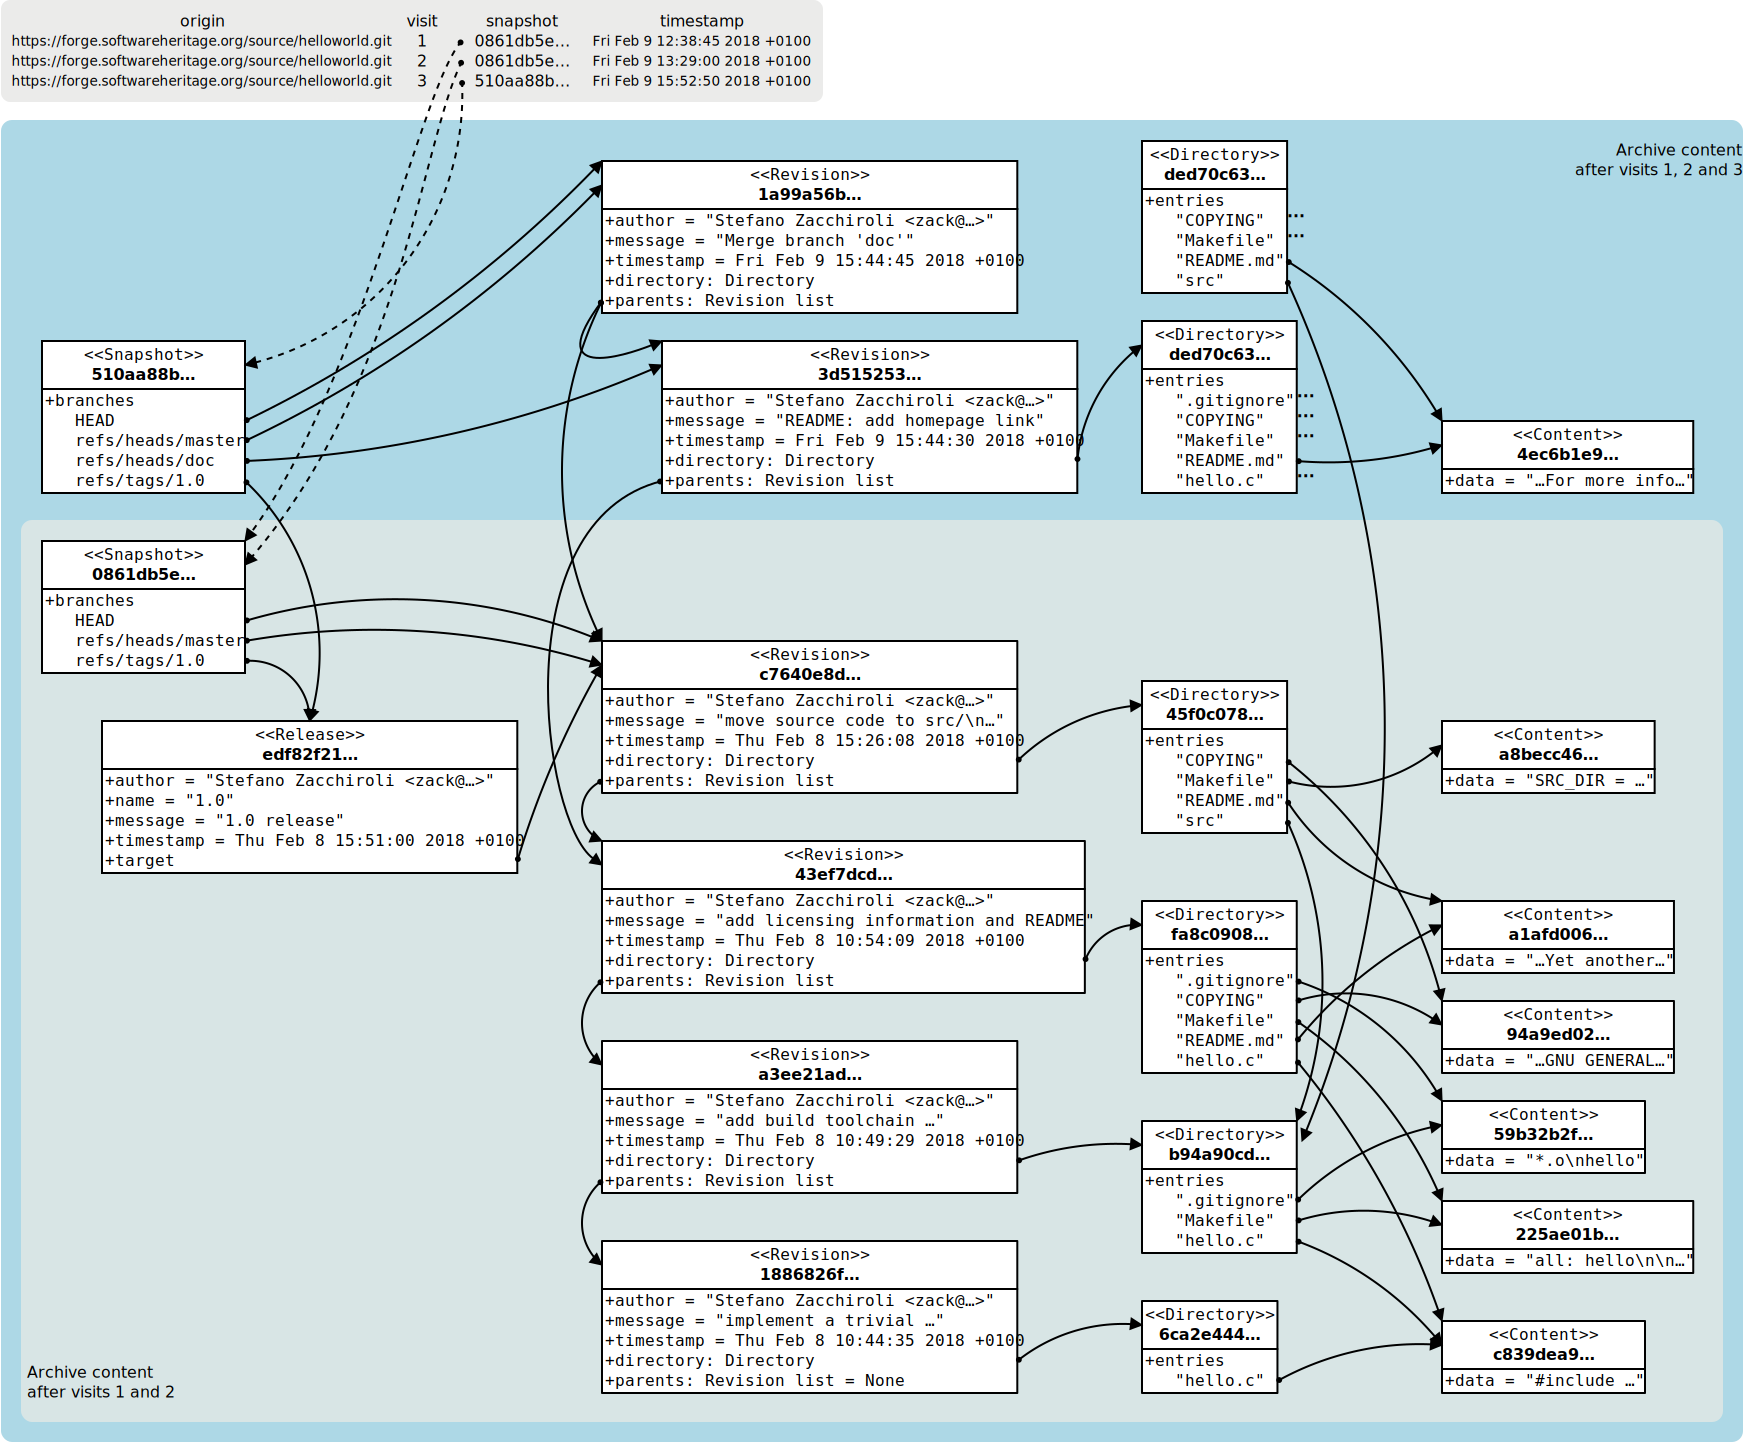
\includegraphics[height=7.5cm]{../img/swh-merkle-dag}
        \end{figure}
    \end{frame}

    % vcs
    % archive

    \section{Making Software Data Available for Mining}

    \section{Graph Compression and Exploitation}

    \section{Graph Topology of Software Development}

    \section{Identification of Software Forks}

    \begin{frame}
        \frametitle{Title}

        \begin{block}{test}
            \begin{itemize}
                \item test
            \end{itemize}
        \end{block}
    \end{frame}

    \section{Conclusion}

    \begin{frame}
        \frametitle{Title}

        \begin{block}{Test}
            \begin{itemize}
                \item TODO
            \end{itemize}
        \end{block}
    \end{frame}
\end{document}
